\section{Background and Motivation}\label{sec:background}
This section provides background on multi-region databases and the issues of existing geo-distributed transaction protocols. 


\begin{table*}[]
  \renewcommand\arraystretch{1.15}
    \begin{tabular}{cccc} \hline
    System      & Transaction Protocol                                        & Consistency  Models       & Coordination Blocking \\ \hline
    Spanner~\cite{spanner:osdi12}     & Read-write: 2PL + 2PC;  Read-only:   TSO                    & SS        & Yes                         \\
    Calvin~\cite{calvin:sigmod12}      & Centralized coordinator                                     & SS        & Yes                         \\
    Slog~\cite{slog:vldb19}        & CRT: Centralized coordinator;  IRT:   Intra-region Sequencer & SS        & Yes                         \\
    Detock~\cite{nguyen2023detock}      & CRT: Dependency-graph;  IRT:   Intra-region Sequencer        & SS        & Yes                         \\
    Janus~\cite{janus:osdi16}       & Dependency-graph                                            & SS        & Yes                         \\
    Epaxos~\cite{epaxos:sosp13}      & Dependency-graph                                            & SS        & Yes                        \\
    Ocean Vista~\cite{ov:vldb19} & TSO  (Watermark)                                            & SS        & Yes                         \\
    CRDB~\cite{taft2020cockroachdb}        & TSO (HLC)                                                   & SKL & Yes                         \\
    RedT~\cite{zhang2023redt}        & 2PL + 2PC                                                   & Serial.              & Yes                         \\
    Tapir~\cite{tapir:tocs}       & Variant of OCC                                              & Serial.              & No (by aborting IRTs)      \\
    MDCC~\cite{mdcc:eurosys13}        & Paxos                                                       & SI      & Yes            \\  \hline          
    \end{tabular}
    \caption{This table summarizes the state-of-the-art geo-distributed transaction systems in the literature. These existing systems either block  IRTs or enforce the IRTs to abort when the IRTs conflict with an ongoing CRT.}\label{tab:compare}
    \vspace{-5pt}
\end{table*}

\begin{figure}[t]  
    \centering
    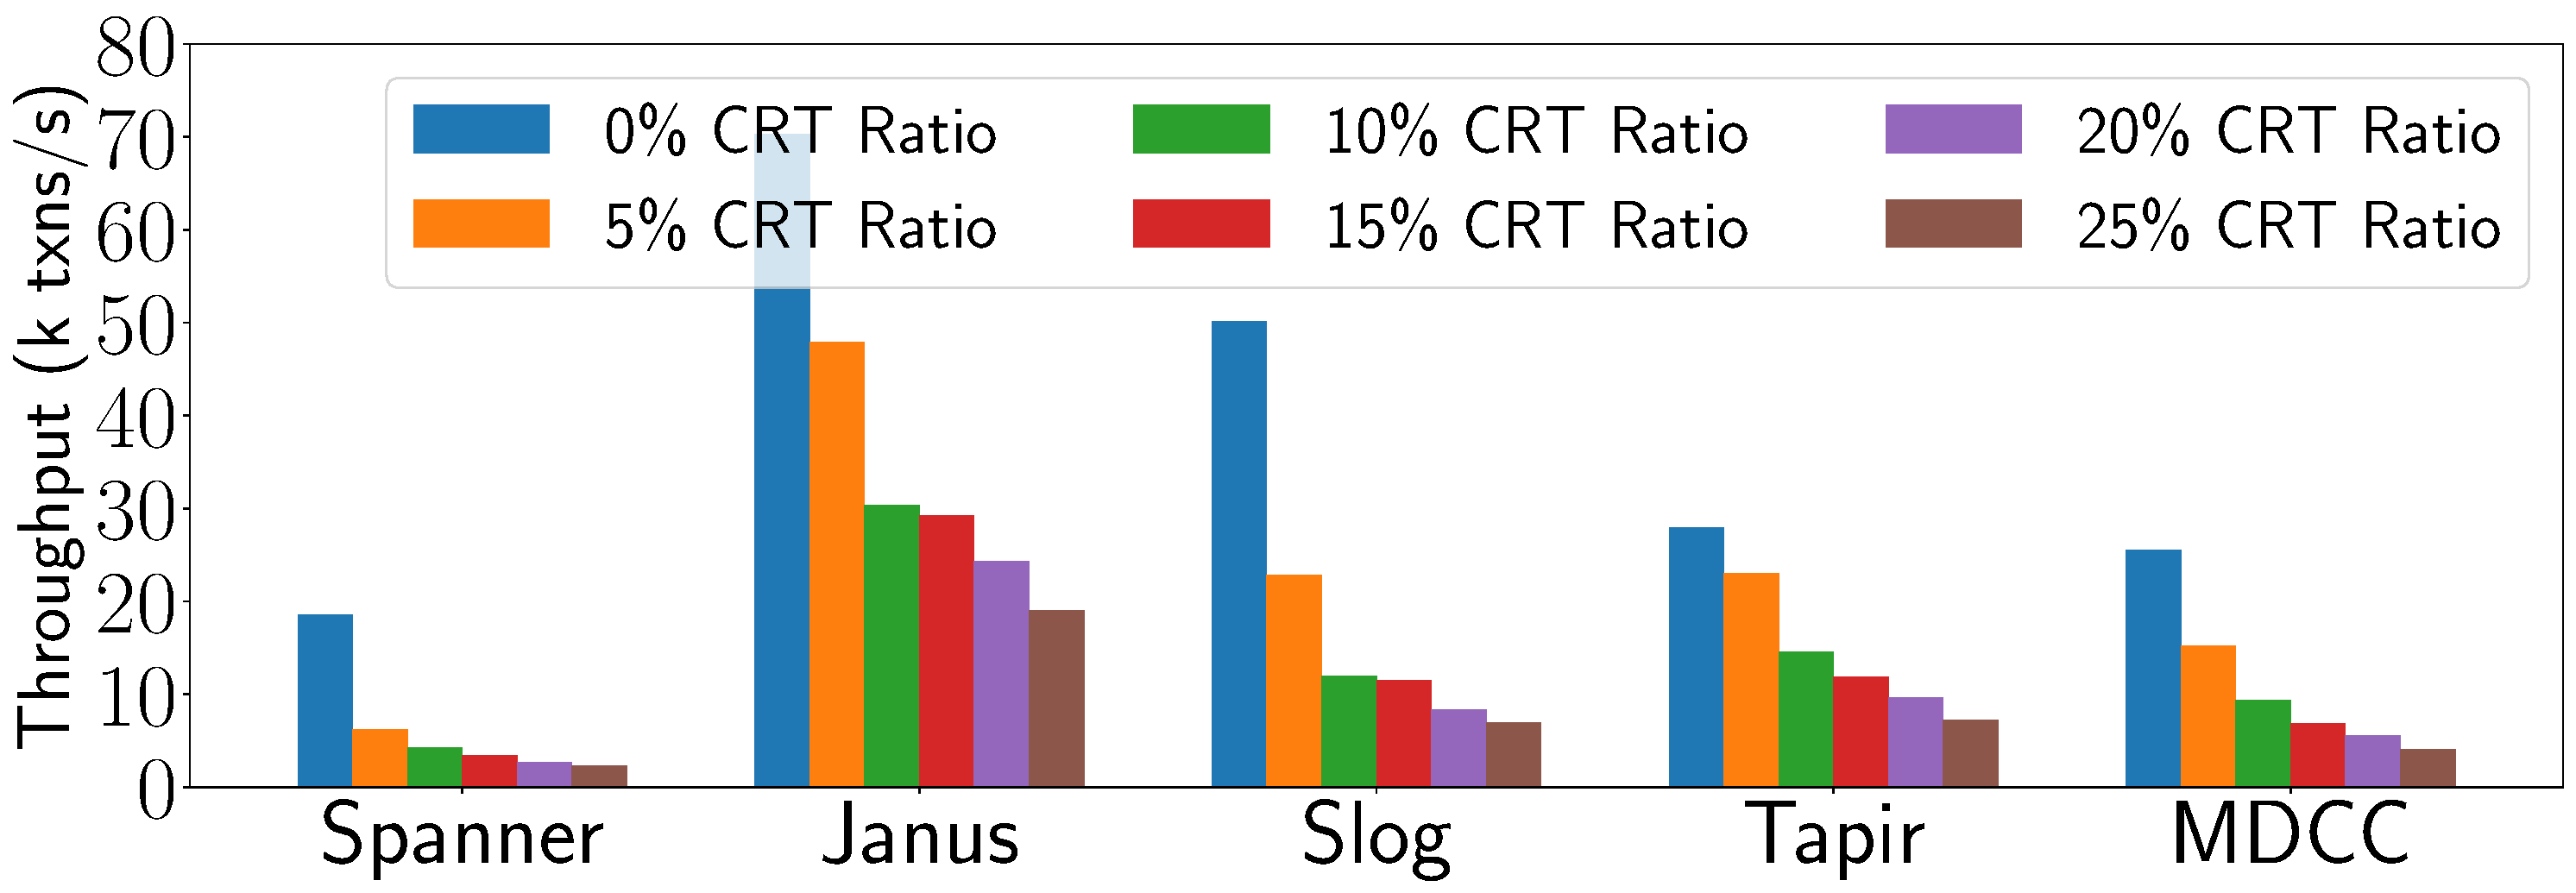
\includegraphics[width=1\columnwidth]{eval-figs/CRT_perf.pdf}
  \vspace{-15pt}
    \caption{Impact of CRT ratio on the throughput of the state-of-the-art geo-distributed transaction systems.}\label{fig:crt}
    \vspace{-5pt}
\end{figure}

\subsection{Multi-region Databases}\label{sec:background:deployment}
Multi-region infrastructures motivate our design of RLS. Deploying a multi-region application has the following advantages. 


\begin{itemize}[leftmargin=*, itemsep=1.5pt]
  \setlength{\itemsep}{0pt}
  \setlength{\parsep}{0pt} 
  \setlength{\parskip}{0pt}
  \setlength{\parindent}{1em}
    \item \textbf{[Low data access latency]} Multi-region deployment enables the placement of data in proximity to active client concentrations across different regions. Applications are designed to predominantly access a data shard from a single region, resorting to cross-region data access only when necessary. This approach facilitates applications in offering global data access with ultra-low latency.
    \item \textbf{[Meet data governance policy]} Privacy regulations impose multi-region deployments for global services with strict requirements on data residency. For instance, the General Data Protection Regulation (GDPR) forbids replicating European citizens' data outside. Thus, multi-region deployments are becoming the de facto choice for multinational companies.
    \item \textbf{[Flexible failure model]} Multi-region deployment allows for data replication across regions, significantly enhancing availability by tolerating complete region failures. In practice, replicating data globally can be costly. Users have the flexibility to define distinct replication policies based on data criticality, such as replicating critical data across regions and keeping other data within the same region.

    

\end{itemize} 



A typical multi-region deployment model is illustrated in \fig{fig:intro}. The database is partitioned into multiple data shards spanning over multiple regions. Each shard comprises a primary replica and several secondary replicas. Replicas can be configured to reside in cross-region or intra-region nodes (servers) based on replication policies. Each region is equipped with a centralized transaction manager responsible for globally consistent metadata (e.g., table schema, data placement policy, and globally unique transaction IDs). Nodes can communicate with each other over the network. Our assumptions include a partially synchronized network, and every message in the database is eventually delivered and processed.
% This new consistency model is especially suitable for emerging mission-critical edge computing applications as this model not only provides strong isolation (i.e., serializability) and real-time order within each region but also has the unique potential of providing stable low latency and availability for single-region transactions (SRT).

\subsection{Geo-distributed Transaction Protocols}\label{sec:background:geo}

Many influential works have been proposed to optimize the performance of geo-distributed transaction processing. We summarize the state-of-the-art systems in \tab{tab:compare}. All of these systems support at least serializability as their consistency model or can be enhanced to serializability with minor modifications (e.g., MDCC).

Generally, these systems focus on optimizing the cost of coordinating transactions from the protocol scope. For instance, some works attempt to reduce either the number or the overhead of network round-trips in transaction coordination. Tapir~\cite{tapir:tocs} improves Spanner's performance by integrating two-phase commit and consensus protocols into a single framework, eliminating redundant coordination and reducing the WAN round-trips. RedT~\cite{zhang2023redt} enhances system performance by further decreasing the network round-trips. RedT targets RDMA-capable networks for local communication and employs a pre-write-log mechanism to eliminate the synchronization of \texttt{prepare} messages (i.e., the first phase in two-phase commits) from the coordinator to primary replicas.


Calvin~\cite{calvin:sigmod12}, Slog~\cite{slog:vldb19}, Detock~\cite{nguyen2023detock}, Ocean Vista~\cite{ov:vldb19}, Epaxos~\cite{epaxos:sosp13}, MDCC~\cite{mdcc:eurosys13}, and Janus~\cite{janus:osdi16} follow the design of deterministic databases, which logically create a global log containing all transactions that have been input into the system. The system then ensures a concurrent execution schedule equivalent to processing all transactions serially in the order they appear in this log (i.e., a partial order). Consequently, after the transaction order is determined, the execution of both CRTs and IRTs can be local. The executors adhere to orders in the logs they receive.

However, all these proposals can not essentially prevent an IRT from being blocked by CRTs (as illustrated in \chref{sec:rls:issue}). Briefly, Spanner and RedT employ two-phase locking for transaction ordering and commit transactions using two-phase commit. When an IRT conflicts with an ongoing CRT, the IRT has to be blocked for the required locks. Tapir uses a variation of OCC and enforces the IRT to abort in the validation phase, resulting in a high abort rate (as confirmed by other previous papers~\cite{ov:vldb19, chen2021achieving}). Determinisct databases either order IRTs and CRTs together (e.g., Calvin, Janus, Epaxos, and Ocean Vista) or require an IRT to be blocked, waiting for the execution of CRTs that are scheduled ahead (e.g., Slog and Detock) for overly strong consistency guarantees.


Consequently, these systems can cause severe performance issues when CRTs occur in the database, and the contention between the IRTs and CRTs is relatively high. We experimentally studied the impact of CRT ratios on the five latest representative systems in \fig{fig:crt}. We used YCSB-T workloads with a Zipf parameter of 0.8. For detailed evaluation setups, we refer readers to \chref{sec:spanner:eval}. From the experimental results, our key observation is that even a few CRTs can significantly degrade the whole system's performance (e.g., up to $86\%$ degradation with only $5\%$ CRTs).



RLS addresses such issues by rethinking the limitations within existing consistency models and thus is fundamentally different from these proposals. RLS trades off consistency for performance with minimal intrusion (i.e., the consistency tradeoff in RLS is tightly necessary for addressing blocking issues). We regard RLS as orthogonal to these advanced geo-distributed transaction protocols. Consequently, new protocols may benefit from the methodology of RLS and the key optimizations of these advanced protocols.